In this section, we will describe the core concepts of a Linux system basic booting process, the basics of security vulnerability discovery and analysis in software, challenges when working with firmware analysis and the basics of re-hosting.  with the main tools that are commonly used in these processes. Later, we will finally present the most common tools used in the process of performing security analysis when working with firmware.

\section{Firmware}

Firmware is a class of computer software that is built for a specific embedded hardware and is critical to this hardware's operation. The goal of a firmware is to provide basic functionalities and act as an operational system for embedded hardware devices. Firmware can be very different from each other and may vary greatly between vendors. Usually a firmware is part of the equipment and is held in the device's non-volatile memory, such as read-only memory (ROM), erasable programmable read-only memory (EPROM), electrically erasable programmable read-only memory (EEPROM) and flash memory. In this research work, we focus our attention in wireless router firmware and most specifically in those who are based on the Linux operating system.

Regarding firmware acquisition for analysis, there are multiple ways to acquire the firmware from a device and the best way to do it will depend on the subject of analysis. For instance, firmware can be extracted from breaking into the physical hardware and finding it's storage device (usually a Secure Digital [SD] card), can also be extracted from the memory dump of a device executing the firmware or even be downloaded from the internet via the vendors website.

For our research, as router firmware (and it's updates) images are usually available in vendor websites and also because we are focusing on scalability, our firmware acquisition process will be focused on downloading firmware images from router manufacturers websites.

\subsection{Linux Simplified Boot Process}

The system startup process depends on the actual hardware the operating system is being booted on. In a personal computer, usually the booting begins in the Basic Input/Output System (BIOS) at a specific address. After that, BIOS search for Linux drives that can are active and bootable. It then calls the bootloader (program that resides in the partition of the boot device - usually a hard disk drive [HDD] for personal computers and an SD card for embbeded computers). The bootloader is then responsible to load the kernel. For personal computers, the bootload can even provide the user the possibility to select which kernel to boot (allowing dual boot for instance). To boot the kernel, the bootloader loads the kernel image and also loads a file known as {\tt initrd} into memory.

Kernel images are commonly a compressed binary file (usually {\tt zImage} or {\tt bzImage} formats) that were compressed using the common {\tt zlib} software library. When loading the kernel, the bootloader decompresses the kernel image and loads it into memory.

Next, the bootloader then loads the initial-RAM-disk (the {\tt initrd} file) into memory and mounts it. It serves as a root filesystem to allows the kernel to boot without requiring any physical disk attached to the hardware. After the kernel is successfully booted, then the root {\tt initrd} is unmounted and the root filesystem is moves to the real filesystem.

For Linux systems running on embedded hardware, the BIOS and the bootloader are commonly replaced with a single program that does the initial hardware setup and then loads the kernel. For instance, one popular program used as a BIOS and bootloader for embbeded devices is the U-Boot bootloader\footnote{\url{http://www.denx.de/wiki/U-Boot}}.

After successful kernel boot, the Linux system finally starts to load userspace applications. The boot process from here on can vary a lot depending on the operating system in question, specially when dealing with embedded hardware. When dealing with Linux for desktop systems, the first started application is usually the {\tt /sbin/init} file. This starts the initialization daemon that in the sequence uses the information contained in the {\tt /etc/inittab} configuration file to perform the last operation of the boot process, that consists of loading programs. After the execution of the instructions in the {\tt /etc/inittab} file, boot process is considered complete and the Linux system is ready to operate.

\section{Re-Hosting}
\label{sec:rehosting}

Re-hosting specifies that a binary that would run on a specific hardware is instead executed on a host system using system emulation and is therefore ``re-hosted'' \cite{firmware-challenges}. Firmware re-hosting in this context relates to executing the firmware, that was originally designed to run on the original hardware, on a desktop computer (i.e. not in the physical hardware it was designed to). Re-hosting challenges involve executing binaries that were designed to run on a specific processor architecture on another. This is usually done using an emulator software.

One very popular open source tool for architecture emulation is the QEMU \cite{qemu} framework, that does dynamic binary translation: guest central processing unit (CPU) instructions are converted to the host CPU instructions, ``translating'' them to work with the change in CPU architecture. QEMU is a complex tool that implements a lot of optimizations to this translation process. It also leverages Linux kernel features from the host (if available) - for instance the Kernel-based Virtual Machine (KVM) - to enhance emulation speed.

QEMU can be used both in ``system emulation'' mode and ``user mode emulation''. In ``system emulation'' mode, QEMU provides the virtual model of a machine, containing CPU, memory to the guest operating system (OS). When executed in ``user mode emulation'' on the other hand, QEMU can execute a process that was compiled for one CPU architecture onto another CPU architecture by emulating the CPU. In short, ``user emulation mode'' is designed to emulate single binaries while ``system emulation'' allows for emulating whole systems.

\section{Software Vulnerability}

Although there are many ways to describe a software vulnerability, one that is close to the software engineering field is that a software vulnerability is an instance of a mistake in the specification, development or configuration of software such that its execution can violate the explicit or implicit security policies \cite{vuln-discovery}. By this definition, one mistake can incur in different vulnerabilities inside a software product.

Companies have put increasingly effort on the adoption of secure software development techniques in early stages of product implementation in order to avoid making mistakes that can lead to vulnerabilities. Even so, software development is a really extensive task and even experienced developers can sometimes make mistakes.

Software vulnerabilities may be exploited by malicious actors to gain access to damage a product or to gain access to sensitive information. Therefore, it is important for companies and security researchers to have effective ways to find vulnerabilities within their products, so that they can update the product to patch these vulnerabilities and provide more security to their business and to their customers. Efficiency in this process is also highly desirable as the latter vulnerabilities are discovered, it becomes more and more expensive to remediate them \cite{soft-eng-economics}.

\subsection{Vulnerability Discovery}
\label{subsec:vuln-disc}

Given the importance of the vulnerability discovery process, some techniques were developed to assist human specialists in this process and these techniques are moving towards becoming more and more automated, such as in the future we may have complete Cyber Reasoning Systems (CRS) working in this process of vulnerability disclosure \cite{crs}.

Nowadays, human specialists are still the main source of vulnerability discovery and the main techniques used in this process are: static analysis, dynamic analysis, symbolic execution and fuzzing. In the following subsections, we will briefly explain how each of these techniques work, and in Table \ref{tab:disc-techniques} we compare these techniques \cite{fuzzing}.

\begin{table}[h]
    \centering
    \caption{Comparison between vulnerability discovery techniques}
        \begin{tabular}{|c|c|c|c|}
        \hline
        \textbf{Technique}   & \textbf{Initial Complexity} & \textbf{Accuracy} & \textbf{Scalability} \\ \hline
        Static Analysis    & Easy      & Low   & Good         \\ 
        Dynamic Analysis   & Hard      & High  & Uncertain    \\ 
        Symbolic Execution & Hard      & High  & Bad          \\ 
        Fuzzing            & Easy      & High  & Good         \\ \hline
        \end{tabular}%
    \label{tab:disc-techniques}
\end{table}

\subsubsection{Static Analysis}

Static analysis consists of searching for vulnerabilities in a software without really executing its code. Static analysis is performed by searching the source code (it can be the object code too, but is a lot harder) for known syntax that may lead to bugs. Static analysis can be automated and tools can be quickly used to search inside a codebase for semantics that appear to be vulnerable. The downside of static analysis is that its simplistic approach is prone to result in a lot of false-positives, and it requires some specialist to read the automated reports to filter the results.

As this analysis is easily automated and quick to execute, it is best used during the development process, and may be even incorporated to the software production pipeline.

\subsubsection{Dynamic Analysis}

In contrast to static analysis in which the software is not executed, dynamic analysis is the process of searching for vulnerabilities in a software during its execution. Software state and execution flow can be monitored during software execution, and a human specialist with strong technical skills in analysis can use this monitored execution environment to find bugs precisely. That being said, this technique is extremely accurate, but also very dependent on the intervention of a human with strong technical skills, restraining the automation of this kind of analysis.

\subsubsection{Symbolic Execution}

Symbolic execution can be considered a specific form of automated dynamic analysis in which the program is executed in a controlled and instrumented environment and each input read by the program is treated as a symbol. When the assembly code reaches a branch instruction that depends on the value of this symbol, then the program takes note of each value constraints for each symbol. This way, knowing every symbol and constraint equation, a symbolic solver could be used to map values for the symbols in such way that every code flow is reached.

This method has been proven to be extremely accurate in small, simple programs. However, when the code grows, the symbolic execution faces the \textit{path explosion} problem. The number of possible paths becomes so big that it becomes impossible for the solvers we have available to calculate every execution flow.

Figure \ref{fig:symbolic-execution} shows a diagram illustrating how symbolic execution works for a sample code.

\begin{figure}[H]
    \centering
    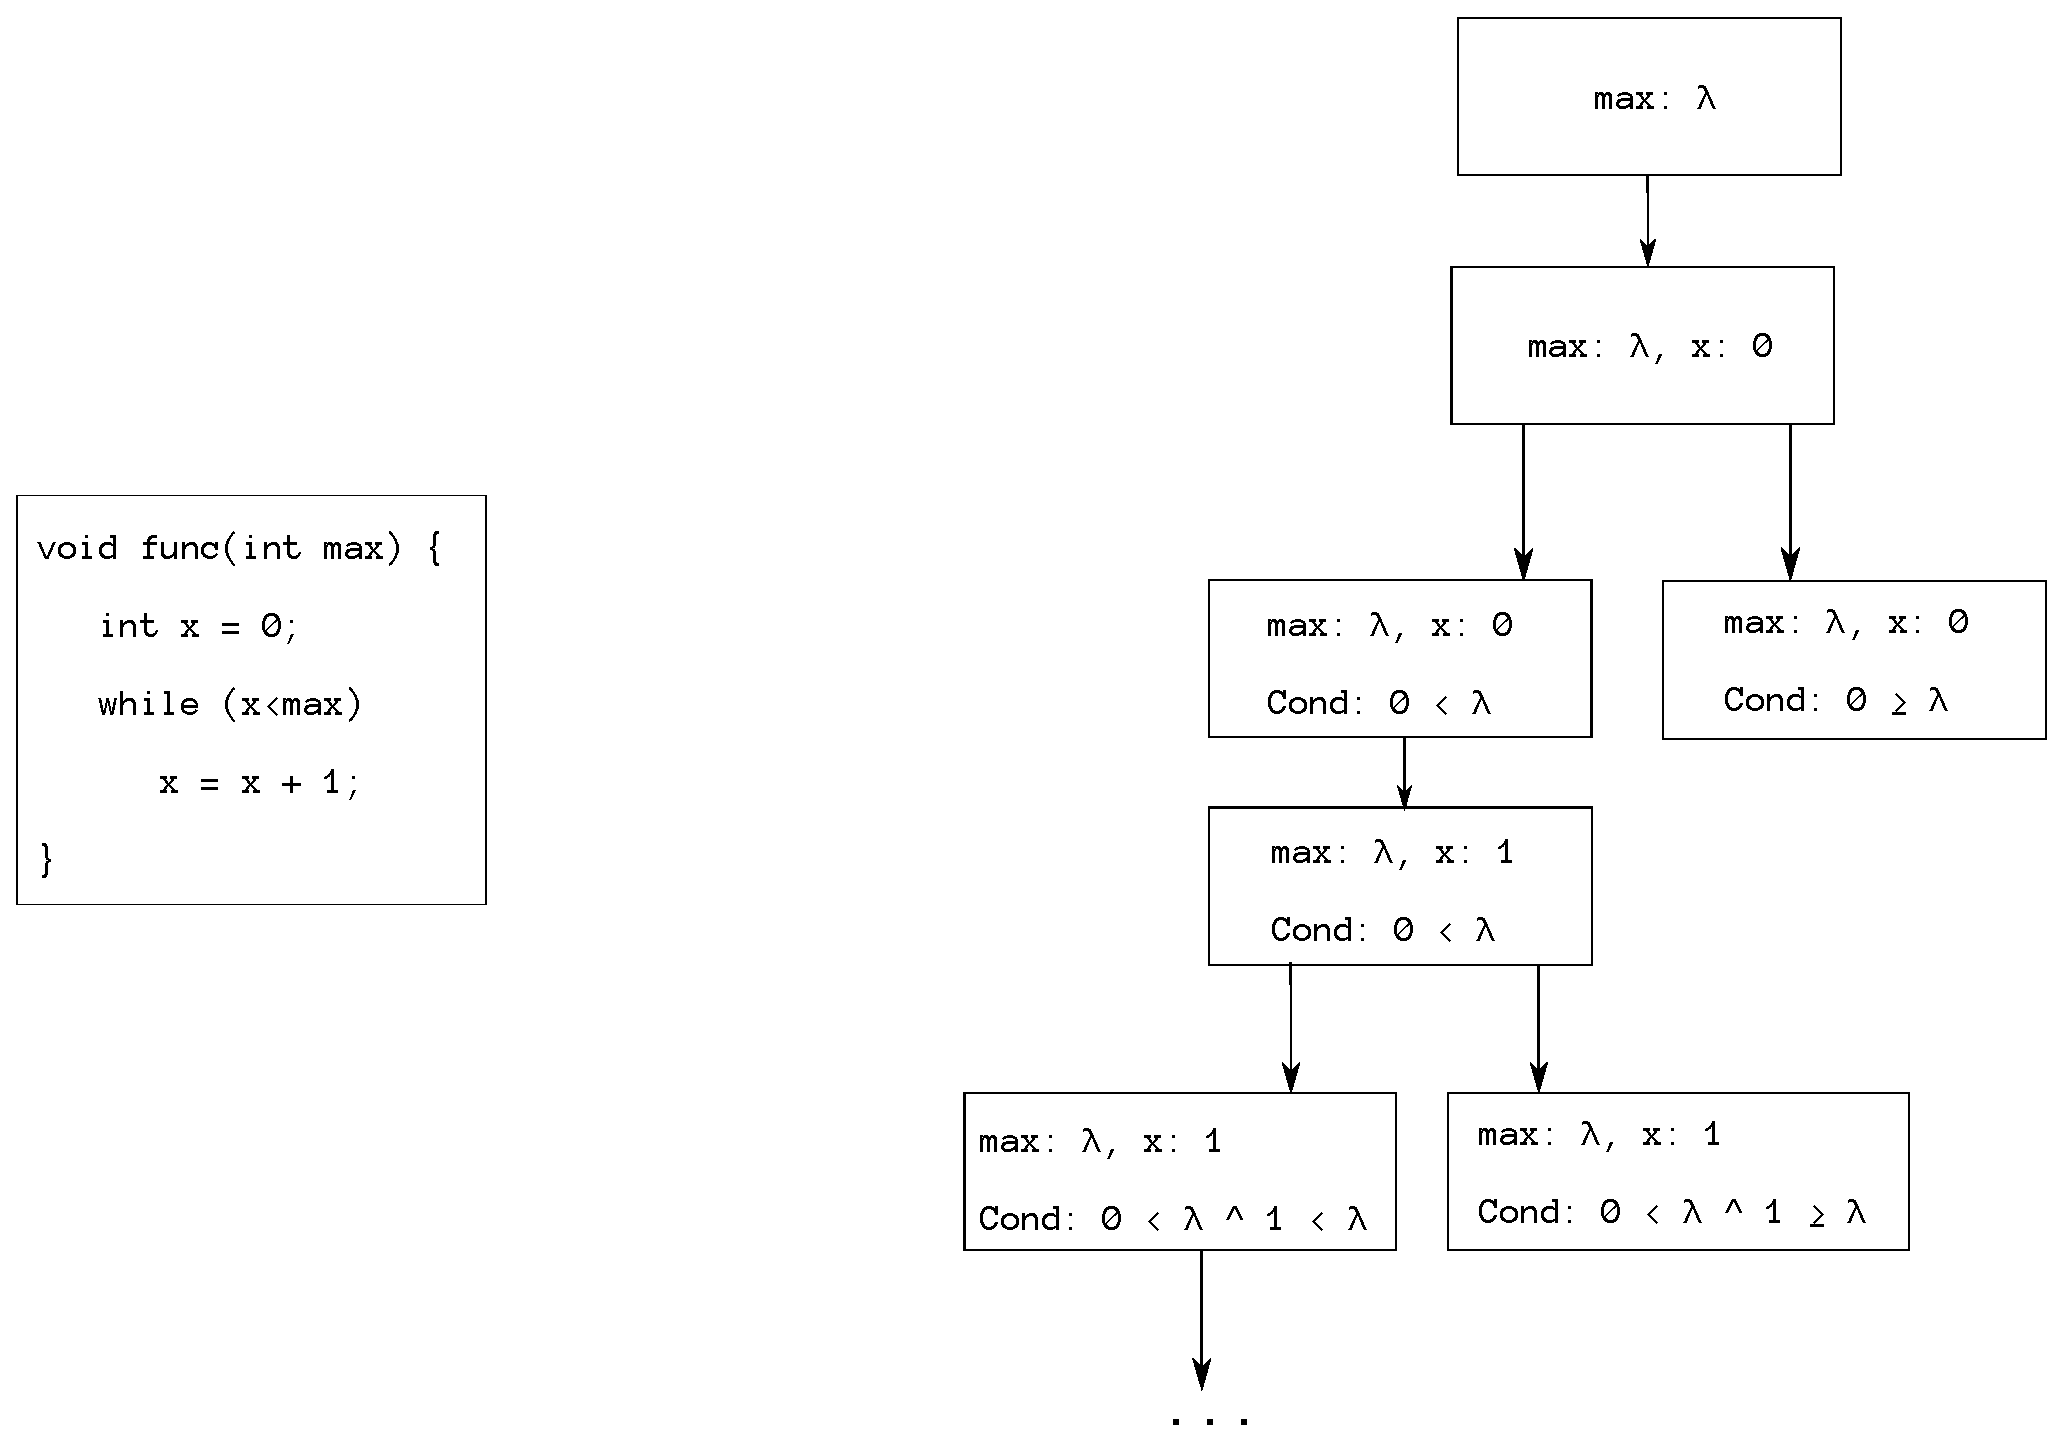
\includegraphics[width=0.8\textwidth]{figs/symbolicalle.eps}
    \caption{Example of a execution tree being constructed during symbolic execution for a sample code (variables being treated as a symbol  - symbol $\lambda$ in the Figure).}
    \label{fig:symbolic-execution}
\end{figure}


\subsubsection{Fuzzing}

Fuzzing can also be considered a specific form of an automated dynamic analysis. This technique consists of generating a massive amount of normal and abnormal inputs and feeding the target program with these generated inputs. Execution state is then monitored to identify if any of the inputs corrupted the execution flow. Fuzzing technique is easy to be deployed, with high accuracy as it is done in the real execution, and also easy to be scaled. However, fuzzing still has issues with low efficiency and code coverage, but as it is also a relatively new technique, a lot of research is being developed upon enhancing this technique, that has already become the state-of-art vulnerability discovery technique currently \cite{fuzzing}.


\subsection{Challenges in Vulnerability Discovery for IoT}

Regarding the vulnerability discovery methods presented in section \ref{subsec:vuln-disc}, these methods were developed to find vulnerabilities in general purpose computers such as home computers or servers. When trying to discover vulnerabilities in software developed for embedded hardware, researchers may face additional challenges~\cite{real-or-rehosted}.

The first challenge may be the acquisition of the target software. Many firmware images were only developed to work within their original hardware, and the only way to have a copy of the software may be opening the physical hardware and extracting the original system from one of its memories.

Another challenge is the dependency of the hardware. Firmware images are usually tied to the original hardware they were designed to operate with. To apply vulnerability discovery techniques in firmware files, we have to re-host the firmware so that it can be run inside an emulator and there we can apply the vulnerability discovery techniques. Usually, re-hosting is a process with a lot of challenges by its own~\cite{firmware-challenges}.

An additional challenge presented by firmware images that don't use a general purpose operating system (such as Linux, FreeRTOS, VxWorks) or firmware files that are really lean is that the vulnerability discovery methods aforementioned rely on monitoring operating system calls that indicate memory corruption. If the firmware don't implement security mechanisms that indicate memory corruption, it becomes a lot harder to automatically detect that the firmware execution reached an abnormal state (caused by the exploitation of an existent vulnerability) \cite{wycinwyc}.

\subsection{Tooling}

In this section, we will present the most common software tools used for firmware analysis and re-hosting. Most work produced relating to firmware analysis and re-hosting makes extensive use of the tools that will be mentioned here and therefore it is important to have an overall understanding about these tools.

\subsubsection{ {\tt binwalk} }

Binwalk \cite{github:binwalk} is a software with the purpose to identify and extract files from inside binary images. It was specifically developed to extract files and code embedded on firmware files, but it also became a popular tool for computer forensics and amongst players of computer security competitions (also known as Capture the Flag competitions). Binwalk achieves that by ``walking'' the binary image looking for magic numbers (file-type signatures). When a magic signature is found, then Binwalk has also the ability to try to extract the found file from inside the binary file. Table \ref{tab:magic-numbers} shows examples of file signatures (magic numbers) for common file-types.

\begin{table}[h]
\centering
\caption{Example of file-type signatures (magic numbers).}
\resizebox{\textwidth}{!}{\begin{tabular}{|c|c|c|}
\hline
\textbf{Hexadecimal Value}                                 & \textbf{ASCII Representation}                & \textbf{File-Type}                   \\ \hline
{\tt \footnotesize 89 50 4E 47 0D 0A 1A 0A}                & {\tt PNG}                     & Portable Network Graphics (PNG Image)\\
{\tt \footnotesize 4C 5A 49 50}                            & {\tt LZIP}                    & LZip Compressed File                 \\
{\tt \footnotesize 7F 45 4C 46}                            & {\tt ELF}                     & Linux Executable File (ELF)          \\
{\tt \footnotesize 25 50 44 46 2D}                         & {\tt \%PDF-}                  & PDF Document                         \\ \hline
\end{tabular}}
\label{tab:magic-numbers}
\end{table}


Binwalk is commonly used in most work related to firmware analysis, and it is usually the first tool used for firmware extraction. Binwalk also provides a Python application programming interface (API) that can be used to integrate Binwalk functionality inside a Python code.

In our work, a script originally developed for the Firmadyne \cite{firmadyne} making extensive use of the Binwalk API was slightly modified to extract the kernel and filesystem from the acquired firmware images.

Just out of curiosity, Binwalk was developed as an open source project in 2010. In 2017 the team behind Binwalk founded a company called ReFirm Labs and launched a commercial closed source version of the tool: Binwalk Enterprise. In early 2021, Microsoft acquired ReFirm Labs and is integrating the commercial version of the tool in it's Azure Defender for IoT product \cite{microsoft-refirmlabs}.

For our future research projects, our team inquired Microsoft about the Binwalk Enterprise pricing. The company was eager to make a cooperation and let our team participate in an early private preview of the Azure Defender for IoT product although we haven't used any of the mentioned commercial tools in this present work.

\begin{figure}[H]
    \centering
    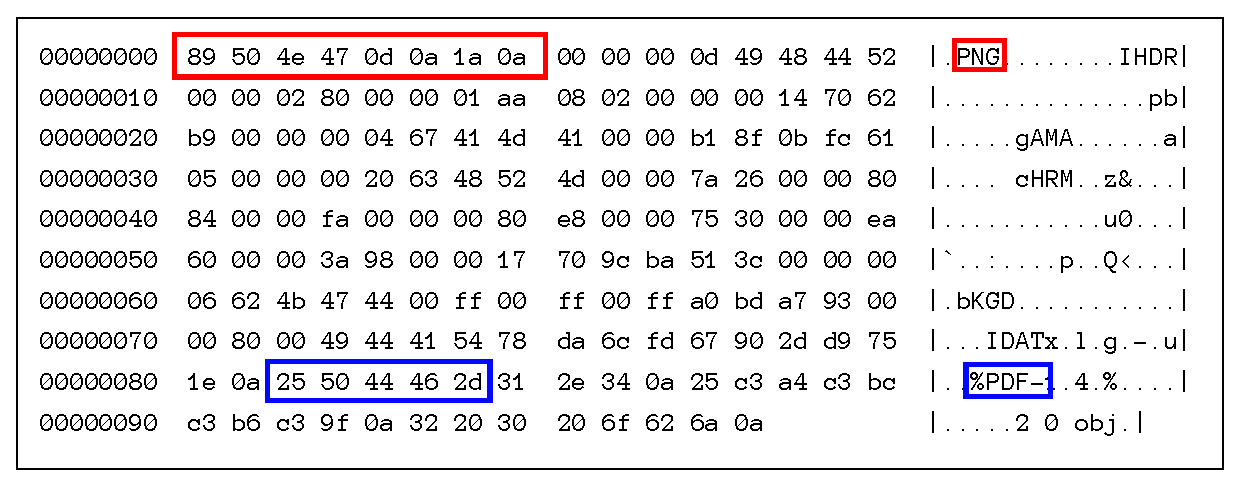
\includegraphics[width=0.7\textwidth]{figs/binwalk.eps}
    \caption{Example of magic numbers being found inside a binary file hexadecimal dump (commonly referred to as a file {\tt hexdump}). From this sample binary, Binwalk would be able to detect and possibly extract a Portable Network Graphics (PNG) image and a Portable Document Format (PDF) document.}
    \label{fig:binwalk}
\end{figure}


\subsubsection{ {\tt dd} }

The {\tt dd} software is part of the GNU Project and it is a command-line utility whose purpose is to convert and copy files for Unix-like operating systems. {\tt dd} is commonly used in firmware analysis for extracting files from a binary file. For most cases, Binwalk may be sufficient and most useful for identifying and extracting data from binary files. When Binwalk fails to extract a file (usually because the firmware is compressed in a way Binwalk can't recognize), {\tt dd} is a great tool to be used to perform the extraction manually.

\subsubsection{ {\tt QEMU} }
\label{sec:qemu}

QEMU \cite{qemu} is an open source machine emulator and virtualizer. It was designed to be a fast machine emulator and it works via binary translation. QEMU is capable of emulating several CPU architectures. As already mentioned in Section \ref{sec:rehosting}, QEMU can be used both in the ``user mode emulation'' to execute single binaries or in the ``system emulation'' mode, in which it can emulate a complete virtual machine.

In our work, as in most research we analysed, QEMU will be the main tool responsible for the re-hosting phase of our idealised architecture, in which it will ideally be used to emulate firmware execution outside it's original hardware, allowing us to dynamically analyse firmware execution and search for vulnerabilities.

\subsubsection{ {\tt Firmware-mod-kit} }

The {\tt Firmware-mod-kit} \cite{google-code:firmware-mod-kit} is actually a wrapper around the already mentioned {\tt dd} and Binwalk tools alongside other tools capable of extracting other types of filesystems that are not already contemplated by Binwalk. Although {\tt Firmware-mod-kit} was not used in our research project, it is not rare to see this tool in firmware analysis articles being used to extract and rebuild linux based firmware and because of that we decided it was worth mentioning it's existence. However, for more actual works, the tool is lacking recent support and we do not advise it usage.

\subsection{ Metasploit Framework }

The Metasploit Framework~\cite{github:metasploit} is an open-source tool designed to develop and execute exploits against a remote computer target. The Metasploit Framework holds a database of publicly disclosed and well known vulnerabilities for popular software, together with pre-configured exploit code that can be used to perform simple, low effort and automated attacks against vulnerable software.

The Metasploit Framework is not actually a common tool used when working with firmware, but it is a common tool used in security analysis. Some of the related work mention the Metasploit Framework tool, and we are also going to mention it furthermore in our work, so that's why we decided to also mention this tool in the tooling section.